This chapter aims to put this report in context by providing a brief overview of some of the central concepts of the \Gls{barricelli} computer.

\section{MIMD Computing}

\Gls{barricelli}, the solution computer presented in this report, is a \Gls{MIMD} computer. \Gls{MIMD}, or Multiple Instruction, Multiple Data, is a class of computer architectures involving multiple autonomous computing units executing different instructions on different data.
Thus, a MIMD computer system consists of several fully independent processing units or cores, interconnected in some way.
Each core/processor is able to work fully independently and asynchronously with their counterparts.
Because of this MIMD lends itself quite well to high performance computing through parallelism.

Communication between the different, possibly heterogeneous independent computing units is either done by message passing, or sharing memory between processors.
Computers that solve communication using message passing might not have any shared memory between the processing units at all.
Each processing unit instead holds its own private memory.
This is called a distributed memory model.
Most MIMD computers implement some hybrid memory solution using both shared memory and distributed memory.

A simplified block-level overview of a MIMD computer can be seen in figure \vref{figure:mimd-block-diagram}.
The computer in the figure uses a shared memory model.
In the figure, the blocks labeled PU are individual processing units.


\begin{figure}[H]
\begin{center}
    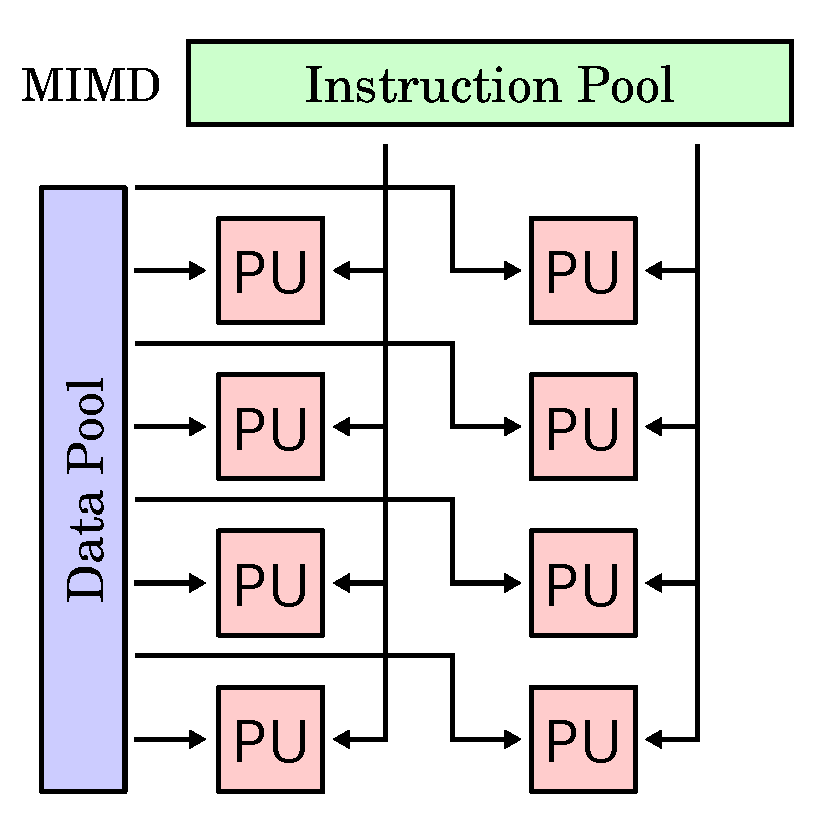
\includegraphics[width=\textwidth/2]{fig/mimd-block-diagram.pdf}
    \caption[
    Block-level overview of a MIMD computer with a shared memory model
    ]{Block-level overview of a MIMD computer with a shared memory model. Reproduced from \url{http://en.wikipedia.org/wiki/File:MIMD.svg}.}
    \label{figure:mimd-block-diagram}
\end{center}
\end{figure}


MIMD architecture forms the basis in the great majority all today’s multi-core super scalar processors.
This is in contrast to the early uniprocessors, which were based on SISD, or Single Instruction stream, Single Data stream. 


Examples of well-known MIMD computing platforms today include Intel's Larrabee platform, and computer clusters connected for instance over the internet.

\section{Genetic Algorithms}
\label{ga-algorithms}

Searching is a well known problem in computer science, because it can be used to solve many other problems.
It is possible to search through a collection of solutions to a problem, rather than finding the correct one by traditional means.
This collection is known as the \Gls{search space}.
It is generally easier to verify that a given solution to a hard problem is correct than finding the solution.
A heuristic search tries to make the search more intelligent than looking at each parameter and comparing it to the other.

A genetic algorithm is a specific type of heuristic search algorithm that is very useful for finding approximate solutions for hard optimization and search problems.
A hard problem in this context is a problem for which there exists no algorithm for feasibly computing a solution within a reasonable amount of time.
In practice, this typically means NP-hard problems.
Classical examples of hard problems for which genetic algorithms can find suitable approximations include the Satisfiability Problem, the Traveling Salesman Problem and the Binary Knapsack Problem, to name a few.
Efficiently finding good approximations to this class of problems is extremely important for many heavy industry processes such as planning and scheduling of processes, finding optimal placement and routing of components in microchip manufacturing, and many other business-critical tasks.


The distinguishing feature of a genetic algorithm compared to other heuristic search algorithms is how it performs its search: it mimics the natural process of evolution to find fit approximations within the search space.
A genetic algorithm represents possible solutions to a given problem as individuals of a population.
The individuals' fitness is calculated by a problem-specific fitness function, and fit individuals are combined together to create new individuals, mimicking the process of natural selection.
The idea is that after simulating a number of virtual generations of individuals, the fittest individual will have survived, and provides a good approximation to the solution.

\subsection{Concepts and Definitions}

To fully understand the inner workings of the \Gls{barricelli}, it is useful to become acquainted with the basic concepts of genetic algorithms.
This subsection of the document defines some genetic algorithm concepts that are used elsewhere in the report.

\paragraph{Experiment}
An attempt at solving a problem using a genetic algorithm.

\paragraph{Individual}
One possible solution (good or bad) to a given problem.

\paragraph{Population}
The group of individuals in a given experiment.

\paragraph{Fitness}
An evaluation of how close an individual is to the theoretically perfect individual.
It is calculated by an objective rating function.

\paragraph{Selection}
Probabilistic selection of rated individuals allowed to reproduce.
The probability of picking a certain individual is typically proportional to its fitness rating.

\paragraph{Crossover}
The combination of individuals (parents) in some way to form a new individual (child).
Also called reproduction.

\paragraph{Mutation}
Mutation of an individual.
It is either random or based on problem-specific rules. 

\subsection{Pseudo-code for a General Genetic Algorithm}

Algorithm \vref{algorithm:pseudo-code-for-ga} shows example pseudo code for a general genetic algorithm.

\begin{figure}[H]
\begin{algorithm}[H]
\SetAlgoLined
\DontPrintSemicolon
\KwData{A population of random individuals}
\KwResult{A quite fit individual}
\Begin{
    $ k \longleftarrow 0 $\;
    $ P_k \longleftarrow $ a population of $ n $ randomly-generated individuals\;
    Compute $fitness(i)$ for each $ i \in P_k $\;
    \While{$ max(fitness(i), i \in P_k) <  threshold $ AND $k < maxIterations $}{
        Selection:\;
        Select $ (1 - x_i) \times n $ members of $ P_k $ and insert them into $ P_{k + 1} $\;

        Crossover:\;
	Select $ x_i \times n $ members of $ P_k $, pair them up, produce offspring, insert offspring into $ P_{k+1} $\;


        Mutation:\;
        Mutate $ \mu \times n $ members of $ P_{k + 1} $\;
	Compute $ fitness(i) $ for each $ i \in P_{k+1} $\;
        $k \longleftarrow k + 1 $
    }
    \Return{the fittest individual in $ P_k $}
}
\caption{Generic genetic algorithm}
\label{algorithm:pseudo-code-for-ga}
\end{algorithm}
\end{figure}


\subsection{Generational Genetic Algorithms} \label{background:generational_genetic_algorithms}
Traditionally, genetic algorithms are implemented with discrete generations \cite{hromkovic}
This means that after a loop in the genetic algorithm, a completely new generation has been created by crossover and mutation.
The original population is replaced with the new one, and the algorithm continues only with the new population.

Generational genetic algorithms can be seen as performing these steps:


\begin{enumerate}
    \item Start with an initial population
    \item Calculate the fitness of each individual in the generation
    \item Selection
    \item Crossover
    \item Mutation  
    \item Loop back to step 2 with a newly created population.
\end{enumerate}

The initial population is normally made from randomly generated individuals.
The diversity ensures that it is possible for the generation to evolve towards a solution without getting stuck in an early local maxima.
In the next stage the fitness of each individual calculated, which is very specific for the problem at hand.
If this fitness values exceeds some specified threshold, the solution is deemed good enough and the algorithm stops.
Note that it will not always find a perfect solution, but one that is sufficient for the problem at hand.
If however none of the individuals end up with a fitness value above the threshold, the algorithm continues.

The solution is found during several phases though a selection, crossover and a mutation phase. 
These phases are used to evolve the population through several generations until an appropriate solution is found. 

The selection step aims to choose individuals for reproduction based on their fitness score, meaning that a higher score gives a higher propability of being chosen.
However, this does not necessary mean that only the fittest individuals are allowed to reproduce.
An important concept of the genetic algorithm is to achieve diversity while exploring the different solutions.
Diversity is important to prevent the algorithm from reaching what is known as a local maximum, a result that has a comparative high fitness score for the immediate region in the \gls{search space}.

A sort of evolutionary dead-end, a stage where the solution found is far from optimal but discovering a more optimal one would require several generations of devolving (selecting individuals with non-max fitness from the current population's descendents).

In the crossover phase individuals from the selection are crossed to produce new individuals.
Because of the initial diversity in the initial population, this will cause the diversity to be large in the beginning.
However they will eventually converge.
The goal of the crossover phase is to converge against a solution by continuously creating a better generation of individuals.
There are several methods for achieving the crossover of individuals, however, the different methods will not be discussed in great detail here.
The different algorithms are highly dependent on the task at hand.
However, the different crossover methods implemented in the employed in the Galapagos architecture will be discussed in greater detail in section \vref{fpga:subsection:genetic_pipeline}.

As a precaution, the individuals are passed through yet another phase: mutation.
The goal of the mutation is to ensure diversity by randomly mutating the individuals by some probability.
The mutation process is usually a simple one that just modifies some of the bits in the individual.
As with the crossover method, algorithms also exist for performing the mutation.


Lastly, it is important to mention that there exists a lot of different classes of genetic algorithms.
They usually employ many different techniques for performing selection, crossover and mutation.
The point of this project is not covering all of them.
In fact, only a subset of problems will be supported on Galapagos architecture.



\subsection{Steady State Genetic Algorithms}
Steady state genetic algorithms do away with the concept of discrete generations.
Rather they continuously select a few individuals, process and return them (or their offspring) to the population.
Older members of the population eventually disappear, based on some selection scheme, preventing the population from growing infinitely large.
This erases the generational border, and has been shown to converge faster towards an optimal solution.
More specifically it allows the algorithm a possible way to work on both rated and unrated individuals at the same time.\cite{steady-state}
This approach is more suited for MIMD architectures, such as the architecture demonstrated in this project.

As steady state algorithms are faster and fitting for MIMD, it was chosen as the main algorithmic goal for the project.


